\documentclass[12pt]{article}

% Preámbulo
%%
\usepackage[T1]{fontenc}
\usepackage[utf8]{inputenc}
\usepackage[spanish]{babel}
\setlength{\parindent}{0cm}
\usepackage[a4paper]{geometry}
\geometry{top=3cm, bottom=3cm, left=3cm, right=3cm}
%%
\usepackage{graphicx}
\usepackage{longtable}
%\graphicspath{c:/Users/Rodrigo/Pictures}
\usepackage{afterpage}
\usepackage{amsmath}
\usepackage{amssymb,amsfonts,latexsym,cancel}
\usepackage{listings}
%\usepackage{minted}
\usepackage{color}
\usepackage{xcolor}
\usepackage{fancyhdr}
\usepackage{hyperref}
\usepackage{multicol}
\definecolor{bg}{rgb}{0.95,0.95,0.95}
\texorpdfstring{}{}
\usepackage{changepage}
\usepackage{subcaption}
\usepackage[absolute,overlay]{textpos}

\lstset{
	language=Python,
	basicstyle=\ttfamily,
	columns=fullflexible,
	showstringspaces=false,
	keywordstyle=\bfseries\color{green},
	commentstyle=\itshape\color{cyan},
	identifierstyle=\color{black},
	stringstyle=\color{red},
}

\hypersetup{
	colorlinks=true,
	linkcolor=blue,
	filecolor=magenta,      
	urlcolor=blue,
}


\renewcommand{\familydefault}{qtm}

\begin{document}
	\title{
		\par\noindent\rule{\textwidth}{0.4pt}
		\textbf{\huge Propuesta del conjunto de datos}
		\par\noindent\rule{\textwidth}{0.4pt}\\{\large PRA 1: Visualización de datos}\\
	}
	\author{Rodrigo Rico Gómez}
	\date{3 de mayo de 2021}
	\maketitle
	\clearpage
	\section{Introducción}
    En este documento se pretende realizar una propuesta de los datos que se utilizarán en la práctica 2. Dicha propuesta se realizará respondiendo a cada una de las preguntas planteadas en la rúbrica de esta actividad, que se encuentra en el campus virtual. Finalmente se presenta una visualización primaria de los datos de forma muy simple.\\
    Los datos que se proponen han sido extraídos de la plataforma \textit{Kaggle} y contienen información acerca de meteoritos caídos en la Tierra. Se recogen datos como su nombre, su masa, su clasificación en la tabla de meteoritos y, lo que es más importante, la localización geográfica de su aterriaje. Los datos han sido publicados por la NASA.
    \section{Relevancia del conjunto de datos}
	\textbf{¿Son datos actuales?}\\
    Al tratarse de fenómenos astrogeológicos, la ventana temporal en la que se encuentran los datos debe ser todo lo dilatada posible, ya que los datos no dejan nunca de ser válidos. A diferencia de otras disciplinas como la sociología, donde la relevancia de los datos depende en gran medida que éstos sean actuales. En este caso, se trabaja con todos los datos disponibles en la historia de la humanidad. La última actualización de estos datos se produjo hace cuatro años.\\
    \\
    \textbf{¿Tratan un tema importante para algún colectivo concreto?}\\
    El estudio de los meteoritos es una rama de la astronomía de la cual se beneficia toda la humanidad.\\
    \\
    \textbf{¿Se ha tenido en cuenta la perspectiva de género?}\\
    Los datos no contienen información que permita hacer una distinción entre el género masculino o femenino de cada registro, se trabaja únicamente con magnitudes físicas, por lo tanto, en este caso no se ha tenido en cuenta dicha perspectiva al seleccionar los datos.
    \section{Complejidad}
    \textbf{Número de registros: Tamaño}\\
    El juego de datos cuenta con más de 45.000 registros. Se considera, por tanto, que el dataset tiene un tamaño aceptable.\\
    \\
    \textbf{Variables disponibles}\\
    Una de las posibles desventajas de este juego de datos es que cuenta únicamente con 10 variables. Sin embargo, se considera que las variables que contiene el juego de datos poseen el suficiente interés como para elaborar una buena visualización. La idea es que el tema principal de la visualización sea la localización geográfica de los meteoritos. A su vez, los meteoritos se caracterizan por la masa y el año en el cual cayeron (o está previsto que caigan) a la Tierra. Evidentemente cada meteorito está identificado unívocamente con un ID y un nombre. Además, el dataset contiene una clasificación de cada meteorito según los criterios de la NASA. De esta clasificación es posible extraer información acerca de la composición y procedencia del meteorito que también puede incorporarse a la visualización. Además, gracias a librerías de Python, es posible decodificar las coordenadas para obtener el país en el cual ha caído el meteorito.\\
    \\
    \textbf{¿Combina variables categóricas y cuantitativas?}\\
    Sí, existen variables categóricas, como la clasificación de los meteoritos realizada por la NASA, el hecho de si han caído ya o no, el país en el que han caído (que se extrae de las coordenadas mediante una librería de Python especializada en tratar datos de geolocalización), y variables cuantitativas como la masa del meteorito o el año de aterrizaje. Otras variables que pueden considerarse cuantitativas son la latitud y longitud, que forman unidas la geolocalización. 
    
    \section{Originalidad}
    Al ser datos de la NASA disponibles de forma abierta, un gran número de personas los han utilizado previamente. Además, al incluir la localización geográfica, son datos que se prestan a elaborar visualizaciones. Si bien es muy probable que ya se hayan realizado visualizaciones previas sobre estos datos, muchas de ellas no son de carácter interactivo. La idea, por tanto, es mejorar las visualizaciones anteriores, creando un mapa sobre el aterrizaje de meteoritos, donde el usuario pueda interactuar con los datos, filtrándolos en base a su masa, clasificación científica, año.
    \section{Las cuestiones que se responderán}
    Como se acaba de comentar, el objetivo es realizar un mapa interactivo de la información. El usuario de la visualización será capaz de navegar a través de los datos respondiendo preguntas como:
    \begin{itemize}
    	\item ¿Cuántos meteoritos han caído en cada país del mundo?
    	\item ¿Cuánto pesa cada meteorito individual?
    	\item ¿En qué año cayó?
    	\item ¿Cómo se clasifican?
    \end{itemize}
    Para responder otras cuestiones ajenas a la localización geográfica, como la distribución de la masa o el tiempo, se acompaña el mapa central con gráficos que reflejen la distribución de estas variables sobre la ventana de datos seleccionados por el usuario. Es interesante la distribución de cada tipo de asteroides en latitud (diferencia entre hemisferios).
    \section{Primera visualización de los datos}
    En la siguiente página se expone una primera visualización básica para ofrecer una primera representación de los datos. No se incluyen en ella todas las variables ni tampoco se pretende responder todas las preguntas, se trata simplemente de una primera toma de contacto con los datos.
    \clearpage
    \begin{figure}
    	\centering
    	\vspace*{-1.5cm}
    	\hspace*{-1.3in}
    	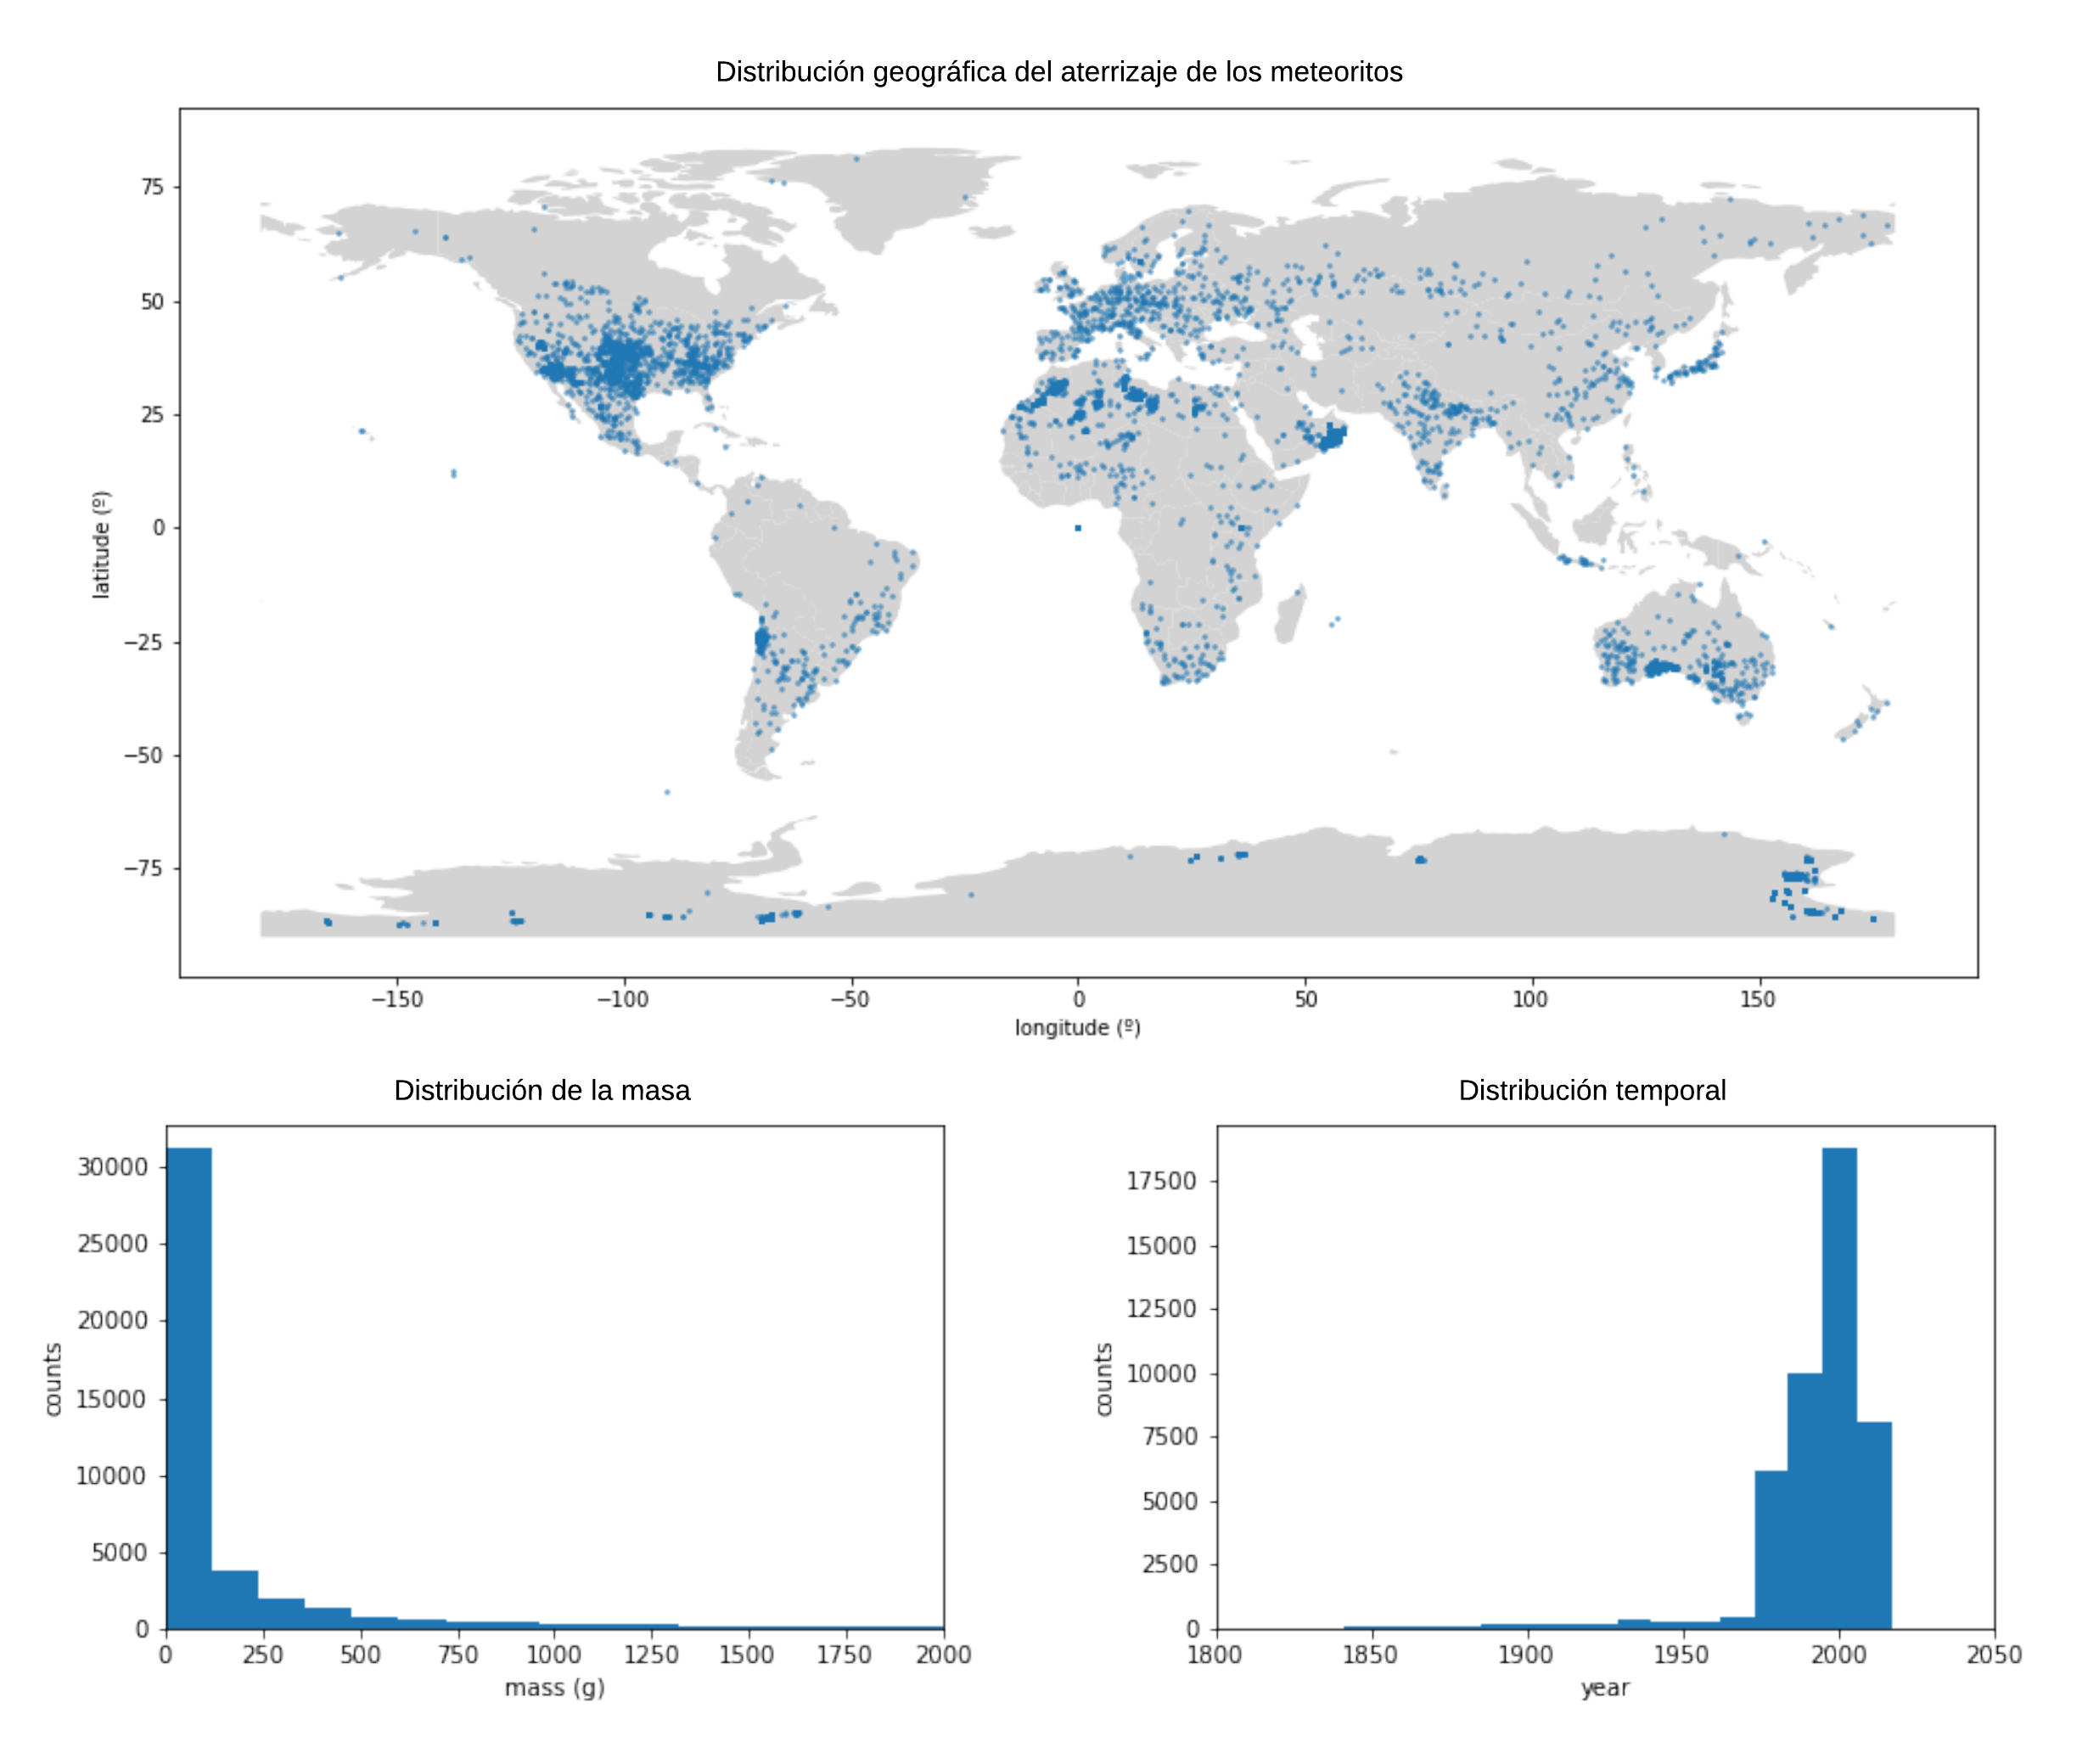
\includegraphics[scale=1.04]{pra1_visualization}
    	\label{rlexample}
    \end{figure}
    
    
	
	
\end{document}